% !TeX encoding=utf8
% !TeX spellcheck = de_DE
% !TeX root = ../Diploma.tex

\chapter{Vergleich zwischen Kotlin und dem Google Web Toolkit}
Ziel dieses Kapitels soll der Vergleich von Kotlin und dem \gls{GWT}. Beide können dazu genutzt werden um JavaScript-Code zu generieren. Dabei ist Kotlin eine Programmiersprache und \gls{GWT} ein Framework, welches in und für die Programmiersprache Java implementiert wurde. Um einen sinnvollen Vergleich zu ermöglichen wird im Nachfolgenden \gls{GWT} in Zusammenhang mit Java bzw. als Erweiterung dieser betrachtet.\\
\\
\todo{Auf nachfolgende Kapitel eingehen}

\section{Vergleichskriterien}\label{sec:comparisonCriteria}
Für die Ermittlung der Vergleichskriterien wurde das Paper \cite{frameworkEvaluation} von Jadhav und Sonar verwendet. In diesem werden zwar Bewertungsmethodiken für Software-Produkte ermittelt und näher erläutert, aber viele dieser Kriterien lassen sich auch auf Programmiersprachen anwenden. \\
\\
Jadhav und Sonar haben dafür, neben der Vorgehensweise eines Vergleichs, die sieben Hauptkriterien aus der \hyperref[fig:comparisionCriteria]{Abbildung~\ref{fig:comparisionCriteria}} entwickelt und anschließend diesen granularere Kriterien zugeordnet. Um eine Bewertung dieser zu vereinfachen wurden noch die Bedeutungen, in Form von Leitfragen, beigefügt.\\
\begin{figure}[htb]
	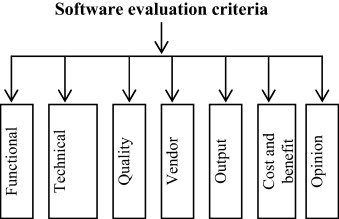
\includegraphics[width=0.5\textwidth]{images/comparision-criteria.jpg}
	\caption{Hauptkriterien des Softwarevergleichs von Jadhav und Sonar \cite{frameworkEvaluation}}
	\label{fig:comparisionCriteria}
\end{figure}
\\
Wie schon Anfangs erwähnt lassen sich nicht alle Kriterien auf Programmiersprachen anwenden, weshalb für diesen konkreten Fall die Kriterien \enquote{Technical} und \enquote{Output} entfallen. Denn mit \enquote{Technical} sind Hardware- und mit \enquote{Output} Ausgabe-Kriterien gemeint, welche in diesem Vergleich keine Anwendung finden.\\
 \\
%Auf Basis des Papers von Jadhav und Sonar wurden die Kriterien, aus der  \hyperref[tab:comparisonCriteria]{Tabelle~\ref{tab:comparisonCriteria}}, für diesen Anwendungsfall ausgearbeitet bzw. angepasst.
 
\subsection{Funktionale Kriterien (Functional)}
\subsubsection{JavaScript-Kompilierung}
\begin{itemize}
	\item In welche JavaScript-Versionen kann kompiliert werden?
	\item Welche Java-Script Modul-System werden unterstützt?
\end{itemize}

\subsubsection{Build-Tools}
\begin{itemize}
	\item Welche Build-Tools werden offiziell unterstützt?
\end{itemize}

\subsubsection{Bibliotheken}
\begin{itemize}
	\item Können schon bestehende JavaScript-Bibliotheken eingebunden werden?
	\item Wie komfortabel ist die Einbindung bestehender Bibliotheken?
	\item Können Java-Bibliotheken eingebunden werden?
\end{itemize}

\subsubsection{Programmierung}
\begin{itemize}
	\item Welcher Programmierstil wird verwendet?
	\item Welcher Grad der Typisierung wird verwendet?
	\item Werden Aspekte der Funktionalen Programmierung unterstützt?
	\item Wie gut ist die Handhabung Funktionaler Aspekte sofern diese existieren?
\end{itemize}

\subsection{Qualitative Kriterien (Quality)}
\subsubsection{Kommunikationsstandards}
\begin{itemize}
	\item Welche gängigen Formate können standardmäßig verarbeitet werden?
	\item Können diese direkt in Objekte geparst werden?
\end{itemize}

\subsubsection{Browser-Support}
\begin{itemize}
	\item Welche Browser werden unterstützt?
\end{itemize}

\subsubsection{Lernkurve}
\begin{itemize}
	\item Wie leicht lässt sich die Programmiersprache erlernen bzw. bedienen?
	\item Gibt es Online-Plattformen um die Programmiersprache auszuprobieren?
\end{itemize}
 
\subsection{Anwenderkriterien (Vendor)}
\subsubsection{Dokumentation}
\begin{itemize}
	\item Gibt es eine ausführliche Dokumentation?
	\item Gibt es offizielle Tutorials?
\end{itemize}

\subsubsection{Support}
\begin{itemize}
	\item Wird Support von Entwicklern angeboten?
	\item Gibt es ein offizielles Forum oder ähnliches?
	\item Auf welchen weiteren Community-Plattformen ist die Programmiersprache vertreten? 
\end{itemize}

\subsubsection{Community}
\begin{itemize}
	\item Wie viele Entwickler sind an der Programmierung der Sprache beteiligt?
	\item Gibt es Unternehmen welche die Entwicklung unterstützen?
\end{itemize}

\subsection{Kosten- und Nutzenorientierte Kriterien (Cost and benefit)}
\subsubsection{Lizenz}
\begin{itemize}
	\item Wurde die Programmiersprache unter einer freie Lizenz veröffentlicht?
	\item Entstehen durch die Benutzung Lizenzkosten?
\end{itemize}

\subsubsection{Benutzungskosten}
\begin{itemize}
	\item Sind kostenpflichtige Programme für die Benutzung notwendig?
\end{itemize}

\subsection{Kriterien an die öffentliche Meinung (Opinion)}
\subsubsection{Beliebtheit}
\begin{itemize}
	\item Wie viele Repositories gibt es auf Github, welche mit der Programmiersprache entwickelt wurden?
	\item Wie viele Fragen wurden auf der Plattform Stack Overflow zu dieser Programmiersprache gestellt?
\end{itemize}

\subsubsection{Veröffentlichung}
\begin{itemize}
	\item Wann wurde die erste Version veröffentlicht?
\end{itemize}

\subsubsection{Indizies}
\begin{itemize}
	\item Welchen Platz hat die Programmiersprache beim Triobe Index belegt?
	\item Welchen Platz hat die Programmiersprache beim RedMonk Index belegt?
	\item Welchen Platz hat die Programmiersprache beim \gls{PYPL} Index belegt?
\end{itemize}
 
%{
%\small\renewcommand{\arraystretch}{1.4}
%\begin{longtabu} to \textwidth{X[1,L]X[1,L]X[2,L]}
%	\captionabove{Kriterien für den Vergleich zwischen Kotlin und dem Google Web Toolkit in Zusammenhang mit Java} \\
%	\hline
%	\taburowcolors 1{tableheadcolor .. tableheadcolor}
%	\bfseries Hauptkriterium &
%	\bfseries Unterkriterium &
%	\bfseries Leitfragen \\ \hline
%	\endfirsthead
%	\hline
%	Hauptkriterium &
%	Unterkriterium &
%	Leitfragen \\ \hline
%	\endhead
%	\hline
%	\taburowcolors 1{white .. white}
%	\multicolumn{3}{r}{\emph{weiter auf der nächsten Seite \ldots}}
%	\endfoot
%	\hline
%	\endlastfoot
%	\taburowcolors 2{tablebodycolor .. tablerowcolor}
%	Funktional (Functional) 
%		& JavaScript-Kompilierung 
%			& In welche JavaScript-Versionen kann kompiliert werden? \\
%			&& Welche JavaScript Modul-Systeme werden unterstützt? \\
%		& Build-Tools 
%			& Welche Build-Tools werden offiziell unterstützt? \\
%		& Bibliotheken 
%			& Können schon bestehende JavaScript Bibliotheken eingebunden werden? \\
%			&& Wie komfortable ist die Einbindung bestehender Bibliotheken? \\
%			&& Können Java-Bibliotheken eingebunden werden? \\
%		& Programmierung 
%			& Welcher Programmierstil wird verwendet? \\
%			&& Welcher Grad der Typisierung wird verwendet? \\
%			&& Werden Aspekte der Funktionalen Programmierung unterstützt? \\
%			&& Wie gut ist die Handhabung Funktionaler Aspekte sofern diese existieren? \\
%	Qualität (Quality) 
%		& Kommunikationsstandards 
%			& Welche gängigen Formate können standardmäßig verarbeitet werden? \\
%			&& Können diese direkt in Objekte geparst werden? \\
%		& Browser-Support
%			& Welche Browser werden unterstützt? \\
%		& Lernkurve 
%			& Wie leicht lässt sich die Programmiersprache erlernen bzw. bedienen? \\
%			&& Gibt es Online-Plattformen um die Programmiersprache auszuprobieren? \\
%	Anbieter (Vendor) 
%		& Dokumentation 
%			& Gibt es eine ausführliche Dokumentation? \\
%			&& Gibt es offizielle Tutorials? \\
%		& Support
%			& Wird Support von Entwicklern angeboten? \\
%			&& Gibt es ein offizielles Forum oder ähnliches? \\
%			&& Auf welchen weiteren Community-Plattformen ist die Programmiersprache vertreten? \\
%		& Community
%			& Wie viele Entwickler sind an der Programmiersprache beteiligt? \\
%			&& Gibt es Unternehmen welche die Entwicklung unterstützen? \\
%	Kosten und Nutzen (Cost and benefit) 
%		& Lizenz 
%			& Wurde die Programmiersprache unter einer freien Lizenz veröffentlicht? \\
%			&& Entstehen bei der Benutzung Lizenzkosten? \\
%		& Benutzungskosten
%			& Sind kostenpflichtige Programme für die Benutzung notwendig? \\
%	Meinungen (Opinion) 
%		& Beliebtheit 
%			& Wie viele Repositories gibt es auf Github, welche mit der Programmiersprache entwickelt wurden? \\
%			&& Wie viele Fragen wurden auf der Plattform Stackoverflow zu dieser Programmiersprache gestellt? \\
%		& Veröffentlichung
%			& Wann wurde die erste Version veröffentlicht? \\
%		& Tiobe Index
%			& Welchen Platz hat die Programmiersprache belegt? \\
%		& RedMonk Index
%			& Welchen Platz hat die Programmiersprache belegt? \\
%		& PYPL
%			& Welchen Platz hat die Programmiersprache belegt? \\
%\end{longtabu}
%}\label{tab:comparisonCriteria}

\section{Vergleichsergebnis}\label{sec:comparisonResults}

\subsection{Funktionale Kriterien (Functional)}
\subsubsection{JavaScript-Kompilierung}
\begin{description}
	\item[Kotlin] Als Ziel der Kompilierung dient der JavaScript-Standard ECMAScript 5. Es existiert aber bereits Pläne für die Umsetzung des ECMAScript 2015 Standards. Für ein Modul-System kann zwischen \gls{AMD}, CommonJS und \gls{UMD} gewählt werden. \cite{kotlinJavaScript, kotlinJsModules} 
	\item[GWT(Java)] Der Standard ECMAScript 5 dient an dieser stelle ebenfalls als Kompilierungsziel. Auch hier ist bereits eine Planung für den ECMAScript 2015 Support bekannt, welcher mit der Version 3.0 veröffentlicht werden soll. Mittels \gls{GWT} ist es nicht möglich ein JavaScript Modul-System zu verwenden. \cite{gwtRoadmap}
\end{description}

\subsubsection{Build-Tools}
\begin{description}
	\item[Kotlin] Es werden gleich eine ganze Reihe an Build-Tools unterstützt. Vertreten sind dabei Gradle, Maven und Ant, wobei die Nutzung von Gradle für die Kompilierung nach JavaScript offiziell empfohlen wird. \cite{kotlinBuildTools, kotlinToJavaScript}
	\item[GWT(Java)] Nur Ant wird unterstützt, aber auch andere Build-Tools wie zum Beispiel Maven oder Gradle lassen sich über Drittanbieter-Software verwenden. \cite{gwtGettingStarted}
\end{description}

\subsubsection{Bibliotheken}
\begin{description}
	\item[Kotlin] Es besteht die Möglichkeit bereits erstellte JavaScript-Bibliotheken, mittels \gls{JsInterop} zu integrieren. Dafür muss die \gls{API} der Bibliothek nachgebaut werden. Da das für große Projekte sehr mühselig sein kann, biete Kotlin dafür das Tool \enquote{ts2kt}\footnote{siehe \url{https://github.com/Kotlin/ts2kt}} an, welches diese Aufgabe übernimmt. Voraussetzung dafür ist nur die Existenz der zugehörigen TypeScript Definitionsdateien. Eine Integration von Java-Bibliotheken ist nicht möglich. \cite{kotlinJsInteop, kotlinJsJavaToJs}
	\item[GWT(Java)] Ebenso wie in Kotlin besteht die Möglichkeit der Einbindung bereits bestehender JavaScript-Bibliotheken, mithilfe von \gls{JsInterop} oder \gls{JSNI}. Aber es wird jedoch nicht mehr empfohlen  \gls{JSNI} zu benutzen, weil diese Technologie veraltet ist und mit der Version 3.0 entfernt wird. Im Gegensatz zu Kotlin können in \gls{GWT} auch Java-Bibliotheken eingebunden, was daher geschuldet ist das generell Java-Code in JavaScript-Code kompiliert wird. \cite{gwtJsInterop, gwtJSNI}
\end{description}

\subsubsection{Programmierung}
\begin{description}
	\item[Kotlin] 
	\item[GWT(Java)] 
\end{description}

\subsection{Qualitative Kriterien (Quality)}
\subsubsection{Kommunikationsstandards}
\begin{description}
	\item[Kotlin] 
	\item[GWT(Java)] 
\end{description}

\subsubsection{Browser-Support}
\begin{description}
	\item[Kotlin] 
	\item[GWT(Java)] 
\end{description}

\subsubsection{Lernkurve}
\begin{description}
	\item[Kotlin] 
	\item[GWT(Java)] 
\end{description}


\subsection{Anwenderkriterien (Vendor)}
\subsubsection{Dokumentation}
\begin{description}
	\item[Kotlin] 
	\item[GWT(Java)] 
\end{description}

\subsubsection{Support}
\begin{description}
	\item[Kotlin] 
	\item[GWT(Java)] 
\end{description}

\subsubsection{Community}
\begin{description}
	\item[Kotlin] 
	\item[GWT(Java)] 
\end{description}


\subsection{Kosten- und Nutzenorientierte Kriterien (Cost and benefit)}
\subsubsection{Lizenz}
\begin{description}
	\item[Kotlin] 
	\item[GWT(Java)] 
\end{description}

\subsubsection{Benutzungskosten}
\begin{description}
	\item[Kotlin] 
	\item[GWT(Java)] 
\end{description}


\subsection{Kriterien an die öffentliche Meinung (Opinion)}
\subsubsection{Beliebtheit}
\begin{description}
	\item[Kotlin] 
	\item[GWT(Java)] 
\end{description}

\subsubsection{Veröffentlichung}
\begin{description}
	\item[Kotlin] 
	\item[GWT(Java)] 
\end{description}

\subsubsection{Indizies}
\begin{description}
	\item[Kotlin] 
	\item[GWT(Java)] 
\end{description}


%\begin{longtabu} to \textwidth {X[L]X[L]X[L]}
%	\captionabove{Vergleichsergebnis zwischen Kotlin und dem Google Web Toolkit in Zusammenhang mit Java} \\
%	\hline
%	\taburowcolors 1{tableheadcolor .. tableheadcolor}
%	\bfseries Leitfrage &
%	\bfseries Kotlin &
%	\bfseries Google Web Toolkit/Java\\ \hline
%	\endfirsthead
%	\hline
%	Leitfrage &
%	Kotlin &
%	Google Web Toolkit/Java\\ \hline
%	\endhead
%	\hline
%	\taburowcolors 1{white .. white}
%	\multicolumn{3}{r}{\emph{weiter auf der nächsten Seite \ldots}}
%	\endfoot
%	\hline
%	\endlastfoot
%	\taburowcolors 2{tablebodycolor .. tablerowcolor}
%	L-1.1 
%		& ECMAScript 5 (ECMAScript 2015 Support ist in Bearbeitung) \cite{kotlinJavaScript}
%			& ECMAScript 5\\
%\end{longtabu}